\documentclass{Interspeech2024}
\usepackage{tipa}
\usepackage{adjustbox}
\usepackage{graphicx}
\usepackage{amsmath}
\usepackage{amssymb}
\usepackage{tikz}
\usetikzlibrary{shapes,arrows}
\usepackage{verbatim}
\usepackage{mathtools}
\usepackage{xcolor}

\usetikzlibrary{calc,positioning}
% 2023-10-21 modified by Simon King (Simon.King@ed.ac.uk)  

% 2024-01 modified by TPC Chairs of Interspeech 2024  

% **************************************
% *    DOUBLE-BLIND REVIEW SETTINGS    *
% **************************************
% Comment out \interspeechcameraready when submitting the 
% paper for review.
% If your paper is accepted, uncomment this to produce the
%  'camera ready' version to submit for publication.

%\interspeechcameraready 


% **************************************
% *                                    *
% *      STOP !   DO NOT DELETE !      *
% *          READ THIS FIRST           *
% *                                    *
% * This template also includes        *
% * important INSTRUCTIONS that you    *
% * must follow when preparing your    *
% * paper. Read it BEFORE replacing    *
% * the content with your own work.    *
% **************************************

% title here must exactly match the title entered into the paper submission system
% \title{Modeling vowel harmony from raw speech using GAN}
\title{Deciphering Assamese Vowel Harmony with Featural InfoWaveGAN}
% the order of authors here must exactly match the order entered into the paper submission system
% note that the COMPLETE list of authors MUST be entered into the paper submission system at the outset, including when submitting your manuscript for double-blind review
\name[affiliation={1,2}]{FirstNameA}{LastNameA}
\name[affiliation={3}]{FirstNameB}{LastNameB}
\name[affiliation={1,3}]{FirstNameC}{LastNameC}

%The maximum number of authors in the author list is 20. If the number of contributing authors is more than this, they should be listed in a footnote or the acknowledgement section.

% if you have too many addresses to fit within the available space, try removing the "\\" newlines
\address{
  $^1$First Affiliation, CountryX\\
  $^2$Second Affiliation, CountryY \\
  $^3$Third Affiliation, CountryZ}
\email{first@university.edu, second@companyA.com, third@companyB.ai}

\keywords{Computational Linguistics, Generative Adversarial Networks, Phonological Learning, Vowel Harmony, Assamese Language}

\newcommand{\red}[1]{\textcolor{red}{#1}}
\begin{document}
\maketitle

% the abstract here must exactly match the abstract entered into the paper submission system
\begin{abstract}
% 1000 characters. ASCII characters only. No citations.
% \noindent Previous well-known models of phonological learning have primarily focused on learning curated text data. We explore whether the Featural InfoWaveGAN model (fiwGAN) can learn iterative long-distance vowel harmony unsupervised when trained on raw Assamese speech data. Assamese is one of the few Indian languages that exhibit phonologically regressive and word-bound vowel harmony. The model produces innovative items by stringing together vowels and consonants from the training dataset and showcases its capability of learning the phonotactics of Assamese along with iterative long-distance harmony with a regressive directionality. A fair number of innovative outputs with non-iterative illicit forms were also generated, suggesting that iterative harmony may indeed be myopic. Our statistical analysis shows that the model prefers a [+high,+ATR] vowel as a trigger throughout the novel items, implying feature learning. We assume that the model takes longer epochs to learn the patterns due to the complexity of vowel harmony and expect that provided more data and a controlled experimental setting, fiwGAN can learn regressive vowel harmony much better. 

\noindent Traditional approaches for understanding the phonology of a language have predominantly relied on curated text data. However, such approaches, although insightful, are limited by the knowledge captured in textual representations of the spoken language. Attempting to overcome this limitation, we investigate the potential of the Featural InfoWaveGAN model (fiwGAN) to autonomously learn iterative long-distance vowel harmony using raw speech data. We focus on the Assamese language, a language known for its phonologically regressive and word-bound vowel harmony. We demonstrate that the fiwGAN is adept at grasping the intricacies of Assamese phonotactics, particularly iterative long-distance harmony with regressive directionality. While the model generates numerous outputs that align with these patterns, it also produces innovative, non-iterative illicit forms, suggesting a degree of myopia in iterative harmony. Our statistical analysis reveals a preference for a specific [+high,+ATR] vowel as a trigger across novel items, indicative of feature learning. We anticipate that with more extensive data and a controlled experimental setup, fiwGAN's proficiency in learning regressive vowel harmony will improve significantly. These findings corroborate the hypothesis on the universality of learning from limited input, innate to humans.

%has to be shortened to 1000 characters
\end{abstract}

\section{Introduction}
Vowel harmony is a phonological phenomenon observed in many languages where vowels within a word tend to be influenced by one another in terms of their phonetic properties, such as tongue height, tongue position, or roundedness \cite{blevins2004evolutionary, rose2011harmony}. Owing to this phenomenon, certain vowels in a word may undergo changes to better match the phonetic characteristics of neighboring vowels. A result is an enhancement of the overall harmony and fluidity of pronunciation within the word \cite{ohala94b_icslp}. Vowel harmony can be categorized as regressive, where vowels are influenced by following vowels, or progressive, where vowels are influenced by preceding vowels.


Among other aspects of grammar, phonology is also a crucial aspect of modeling human acquisition, as it is essential to understand the model's inherent bias and its ability to make human-like generalizations. To address how a grammar derives surface phonetic outputs from phonological inputs, researchers have proposed several learnability approaches, commonly executed as machine-implemented models that mirror the capacities of human children. The Generative approach or the rule-based approach \cite{chomsky_sound_1968} derives outputs from input through derivation. Optimality Theory \cite{prince_optimality_2004}, and other related proposals like Harmonic Grammar and Maximum Entropy Grammar \cite{legendre_can_1990,goldwater_learning_2003,hayes_maximum_2008,pater_weighted_2009} model phonological grammar as an input-output pairing; they choose the most optimal output based on an input. Deviating from the Optimality Theoretic approach, \cite{hayes_maximum_2008} proposed a Maximum Entropy grammar model assuming that the constraints in a grammar are learned from language-specific data and are not universal. The model determines constraints from the input data by choosing the constraints among the candidates. \cite{hayes_maximum_2008} employ machine learning techniques and examine the model's capacity to learn the interacting constraints responsible for English onset projection, Shona vowel harmony, and Warrgamay phonotactics.

In his in-depth assessment of previous generative linguistics research, \cite{pater_generative_2019} argued the significance of implementing neural network approaches. The power of neural models as statistical learners provides a valuable tool for work on the learnability of linguistic phenomena by allowing us to begin determining the upper limit on what is learnable from lexical statistics alone and how different representational assumptions guide this learning \cite{mayer_phonotactic_2020}. The sequence-to-sequence model developed by \cite{kirov_recurrent_2017} and \cite{kirov_recurrent_2018} was trained using the same dataset used in \cite{albright_rules_2003} and predicted a better match to a native speaker. \cite{prickett_learning_2022}'s seq-to-seq model demonstrates that it is possible for a neural network structure without variables to capture the linguistic capabilities of humans. \cite{mayer_phonotactic_2020}'s simple Recurrent Neural Network examined Finnish vowel harmony, Cochabamba Quechua laryngeal cooccurrence restrictions, and English sonority projection datasets. Comparing the results to MaxEnt learner \cite{hayes_maximum_2008}, they show that the neural network architecture captures a learning mechanism similar to human judgments. However, the majority of the existing models (including finite-state automata, MaxEnt grammar, and the neural network models) learn either phonetic or phonological learning at a time, assuming that one of the other has already been achieved by the learner\cite{martin_learning_2013,dupoux_cognitive_2018}. Recently \cite{rasanen_analyzing_2016} and \cite{shain_measuring_2019} reported that a neural network autoencoder learns phoneme-like representations without the need for explicit labeling. \cite{shain_measuring_2019}'s autoencoder model is trained on pre-segmented acoustic data. It inputs the acoustic data and outputs corresponding values to phonological features. Given the autoencoder architecture, the model does not generate innovative data but attempts to match the outputs to the input as closely as possible. 

Generative Adversarial Network (GAN) is claimed to model learnability more naturally as phonetic and phonological processes are computed as the mapping from random space to generative data \cite{goodfellow_generative_2014,begus_generative_2020}. \cite{donahue_adversarial_2018} proposed a WaveGAN model for audio data to learn language features from continuous speech signals based on the DCGAN architecture\cite{radford_unsupervised_2015}. The model takes 1s long audio files as inputs, sampled at 16 kHz with 16-bit quantization. They are converted into vectors and fed to the discriminator network. The WaveGAN model for phonetic and phonological learning \cite{begus_generative_2020} successfully captures the linguistic representations as a one-to-one mapping from latent space to generated data, similar to how humans construct underlying phonological representations by listening to a speech stream in a language. However, a crucial aspect of human acquisition is lexical learning- the ability to store unique information attached to each meaning-bearing unit or phonemes and to generate new lexical items while also conforming to the phonotactics of their language. \cite{begus_ciwgan_2021} modified the WaveGAN architecture by adding a lexical learning component- Q-network \cite{chen_infogan_2016} which enables the Generator to produce linguistically categorically meaningful sounds and named it Featural InfoWaveGAN (fiwGAN)\cite{begus_ciwgan_2021}. FiwGAN has the advantage of proposing a new latent space structure to understand featural representations of phonetic and phonological learning. The Generator network learns how to generate acoustic data that encodes unique lexical information and outputs innovative acoustic data such that each lexical item is associated with a unique binary code. \cite{begus_interpreting_2022} examined the fiwGAN network on English allophonic distribution and argued that the model is not only generative but also learns the conditional allophonic distribution and produces innovative data that can be compared to productive outputs in human speech acquisition. %Further, by manipulating a single variable in the latent space, the model can change the generated token from \#sTV [stop preceded by frication is unaspirated] to \#T\textsuperscript{h}V [aspirated stops at the initial position of a stressed syllable]. 
\cite{chen_exploring_2023} examined the robustness of the fiwGAN model by testing English and French nasality. The results meet \cite{begus_generative_2020}'s claim that the GANs can learn phonological representation where single latent variables correspond to identifiable phonological features. The ability of fiwGAN to distinguish between the English non-contrastive and French contrastive nasality makes the model an adept phonological learner, given it is tested in a more controlled setting in which the same feature is compared across languages. 

\section{Proposed approach}
 Vowel harmony is a complex phonological process. It requires the learner to grasp crucial aspects like directionality, domains, features, iteration, locality, and opacity \cite{archangeli_harmony_2007}. Traditionally, the directionality of harmony is categorized into two parts: progressive/preservatory (left-to-right) and regressive/anticipatory (right-to-left). In Assamese, the [+ATR] (advanced tongue root) vowels trigger harmony of [-ATR] vowels. The dominant feature [+ATR] spreads regressively from both roots and suffixes. The vowel harmony system of Assamese provides a crucial case study for directionality as it is neither stem-controlled nor dominant-recessive \cite{mahanta_directionality_2008}. Assamese also shows iterative long-distance vowel harmony where [+ATR] vowels trigger all the preceding [-ATR] vowels in a word. We examine whether the fiwGAN architecture learns long-distance iterative harmony and regressive directionality. We train the model with Assamese speech data containing both harmonic and non-harmonic words. We analyze the innovative items and observe that the vowels in some of them iterate over a longer domain exhibiting long-distance harmony, and the error items display non-iterative local harmony. We quantify the presence of [+ATR] harmony when the frequency of F1 of the target vowel [-ATR] is much lower in the vicinity of the trigger vowel [+ATR] than respective F2 and F3 \cite{mintz_infants_2018,olejarczuk_acoustic_2019}. Regressive directionality is anticipated when V2 explains the properties of V1 in a V1CV2 setting. We analyze the output audios statistically and observe that although the Generator strings vowels and consonants together to form a novel word, it does follow a vowel sequence within the word domain. We also identify that some innovative items have lexical meaning in Assamese, suggesting the emergence of lexical learning from the fiwGAN model.
 
\section{Assamese}
Assamese is an Indo-Aryan language spoken in the northeastern state of Assam by 15.3 million speakers \cite{census_2011}. The variety discussed for this research is the colloquial Assamese spoken in the eastern region, also known as Upper Assam. Assamese has 8 surface vowels [i, e, \textepsilon , \textscripta, \textopeno, o, \textupsilon, u] and 20 consonants [p, p\textsuperscript{h}, b, b\textsuperscript{h}, t, t\textsuperscript{h}, d, d\textsuperscript{h}, k, k\textsuperscript{h}, g, g\textsuperscript{h}, m, n, \textipa{\ng} s, z, x, h, \textturnr, j, w, l] \cite{mahanta_directionality_2008}.

\begin{table}[!ht]
\centering
\adjustbox{max width=0.45\textwidth}{
\begin{tabular}{lllll}   
\hline
\textbf{Vowels} & \textbf{Front} & \textbf{Back} &  & \textbf{ATR} \\
\hline
High & i &  & u & +ATR \\
 &  &  & \textupsilon& -ATR \\
Mid & e &  & o & +ATR \\
 & \textepsilon &  & \textopeno& -ATR \\
Low &  &  & \textscripta& -ATR \\ \hline
\end{tabular}}
\caption{Vowel inventory of Assamese}
\label{tab:accents}
\end{table}
\subsection{Assamese vowel harmony}
Vowel harmony is a phonological process where adjacent vowels in a word change their vocalic properties to match the neighboring vowels. Assamese is one of the few Indian languages that exhibits rich vowel harmony. \cite{mahanta_directionality_2008} has explicitly studied and more recently, \cite{archangeli_assamese_2020} gave us new perspectives about vowel harmony in Assamese.
The surface vowels' occurrence is restricted in the following ways: 

\begin{itemize}
    \item The two high vowels /i/ and /u/ are pronounced with an advanced tongue root [+ATR], as are the mid vowels /e/ and /o/.
    \item The mid vowels / \textepsilon/ and / \textopeno/ are slightly lower than /e/ and /o/ and are not realized with an advanced tongue root [-ATR].
    \item /e/ and /o/ cannot occur word-finally or initially; they occur only under circumstances of vowel harmony.
\end{itemize} 

\begin{table} [!ht]
  \centering
    \adjustbox{max width=0.45\textwidth}{
    \begin{tabular}{lllll}
    \hline
         \textbf{Assamese} &  \textbf{Gloss} &  \textbf{-suffix} &  \textbf{Harmonised} & \textbf{Gloss} \\
         \hline 
          /p\textepsilon t/&  ‘belly’ &  -u &  [petu]& ‘pot-bellied’ \\
         /b\textepsilon p\textscripta r/&  ‘trade’ &  -i &  [b\textepsilon p\textscripta ri]& ‘trader’ \\
         /z\textupsilon n\textscripta k/ & 'firefly-M' & -i & [z\textupsilon n\textscripta ki] & 'firefly-F'\\ 
         /p\textscripta g\textopeno l/ & 'mad-M' & -i & [p\textscripta goli] & 'mad-M'\\
        \hline
\end{tabular}}
\caption{An example of vowel harmony in Assamese \cite{mahanta_directionality_2008}}
\label{harmonytable}
\end{table}

Assamese exhibits right-to-left ATR harmony where the high vowels /i/ and /u/ trigger [+ATR] harmony of [-ATR] high /\textupsilon/ and mid vowels [/\textepsilon/, /\textopeno/] in the language. Exceptional patterns emerge when a root morpheme containing the vowel /\textscripta/, in suffixes like /-ij\textscripta/ and /-uw\textscripta/, is added. An otherwise opaque vowel [\textscripta] becomes either /e/ or /o/.  From the examples of Table \ref{harmonytable}, we can argue that the stem vowels alternate under the influence of suffixes in Assamese. [+ATR] acts as a dominant feature that spreads from the stem vowels in the leftward direction and affects vowels on the left side of the triggering vowel. As seen in the examples, harmony applies to all the [-ATR] vowels preceding a [+ATR] vowel within the word domain.\cite{mahanta_directionality_2008} proposed that the harmony sequence in the language may be subject to the tendency of avoiding featural cooccurrence of [-ATR, +ATR] vowels. Therefore, [-ATR] vowels do not trigger harmony playing a recessive role. /\textscripta/ appears to be an opaque vowel that blocks harmony from its targeting vowels to its left (z\textupsilon n\textscripta ki 'firefly' *zun\textscripta ki). /\textscripta/ is raised when derivational suffixes [uw\textscripta] and [ij\textscripta] are attached. /\textscripta/ is raised according to the preceding [-ATR] vowel, for example, when the preceding vowel is /\textepsilon/, /\textscripta/ becomes [e] (\textepsilon lah-elehuw\textscripta) and [o] otherwise. \cite{archangeli_assamese_2020} proposed that iterative harmony is gradient and vowels closer to the trigger is affected more than the ones further away from the trigger. Our study attempts to navigate these claims through modeling learnability computationally.

\begin{figure}
    \centering
    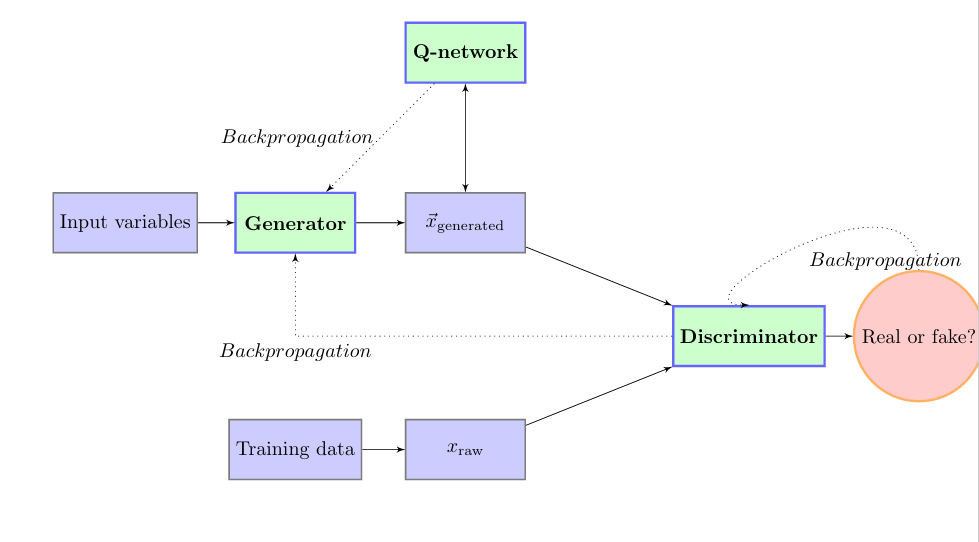
\includegraphics[width=1\linewidth]{fiwGAN.png}
    \caption{An illustration of fiwGAN}
    \label{fig:enter-label}
\end{figure}

\section{Model}
FiwGAN \cite{begus_ciwgan_2021} contains three deep convolutional layers, namely, Generator, Q-network, and Discriminator. In traditional GAN models \cite{goodfellow_generative_2014,donahue_adversarial_2018}, the Generator, a 5-layer convolutional network, takes a set of uniformly distributed latent variables (z $\sim$ U(-1,1)) as input. In fiwGAN, the Generator's latent space consists of binary codes($\phi$) and latent variables. As a result, the network treats binary variables as features where each variable corresponds to one feature ($\phi\textsubscript{n}$)\cite{begus_ciwgan_2021}. The Generator, trained to maximize the Discriminator's error rate and minimize the Q-network's error, outputs a 1D vector of 16,384 data points consisting of about 1-second long acoustic outputs sampled at 16 kHz. These outputs and the real acoustic data are fed to Discriminator, which is trained to calculate the Wasserstein distance \cite{arjovsky_wasserstein_2017} between the generated and the real data. The Q-network, a 5-layer convolutional network, is fed with the same input data as the Discriminator. Contrary to the Discriminator, the Q-network's final layer comprises n nodes corresponding to the number of categorical variables ($\phi$). Q-network's loss function triggers the model to update the weights of the Q-network along with the Generator. This enables the Generator to associate lexical items with a unique latent code so that Q only retrieves the code from the acoustic signals. This system results in lexical learning. The generator outputs raw acoustic data that is never a full replication of the real input data, but it is similar. Figure\ref{fig:diagram} presents how the fiwGAN architecture works when trained on Assamese data.\footnote{We used the model's Pytorch version, which is available at \url{https://github.com/gbegus/ciwganfiwgan-pytorch.git}.}


\section{Materials and methods}

\subsection{Participants and data}
For this experiment, 15 native Assamese speakers (7 males, 8 females) between the ages of 19-35 were consulted. The data was recorded with a Tascam DR-100 MKII recorder in the soundproof booth at the Phonetics and Phonology lab of IIT Guwahati. 
The dataset consisted of 82 words in total. Each target word was in a carrier sentence written in Assamese script ('moi X buli kolu' in Assamese; 'I say X' in English). The participants were asked to utter each word at least four times. This resulted in 5000 tokens; some words were repeated more than four times. The collected speech data was then manually segmented using PRAAT\cite{boersma_praat_2009} for analysis. 

\begin{table}
\caption{Example dataset for training fiwGAN}
\label{tab:accents}
\centering
\adjustbox{max width=0.45\textwidth}{
\begin{tabular}{lll}
\toprule
\textbf{Assamese}& \textbf{suffix}&\textbf{Harmonised} \\
\midrule
\textepsilon lah& -uw\textscripta& elehuw\textscripta\\
\textscripta l\textscripta x& -uw\textscripta& \textscripta loxu\textscripta\\
dil\textepsilon& -i& dilei\\ 
nokoril\textepsilon& -u& nokorileu\\ \bottomrule
\end{tabular}}

\end{table}

\subsection{Method}
The model takes 4789 (3169 harmonic and 1620 non-harmonic) 1-second-long unannotated single-channel audio files sampled at 16 kHz in raw waveforms. The Generator is trained with seven binary latent codes, allowing for 100 uniformly distributed latent variables z (U$\sim$(-1,1)) and 2\textsuperscript{7}=128 unique classes, represented as [1,0,0,0,0,0,0 for word1],[0,1,0,0,0,0 for word2], etc. The model was trained at a .0001 learning rate with a batch size of 64. It ran for three consecutive days on an NVIDIA GPU at the CLST lab of IIT Guwahati. The Generator data was loaded following 960 training epochs ($\sim$ 44000 steps). 64 out of 100 outputs were analyzed for our experiment. 
\begin{figure*}[!t]
    \label{fig:formants}
    \centering
    \begin{tikzpicture}
% ----- row 1: put the images

\node[inner sep=0pt,anchor=center] (main_fig) at (2,20) % {x,y} from left corner in an imagined grid
{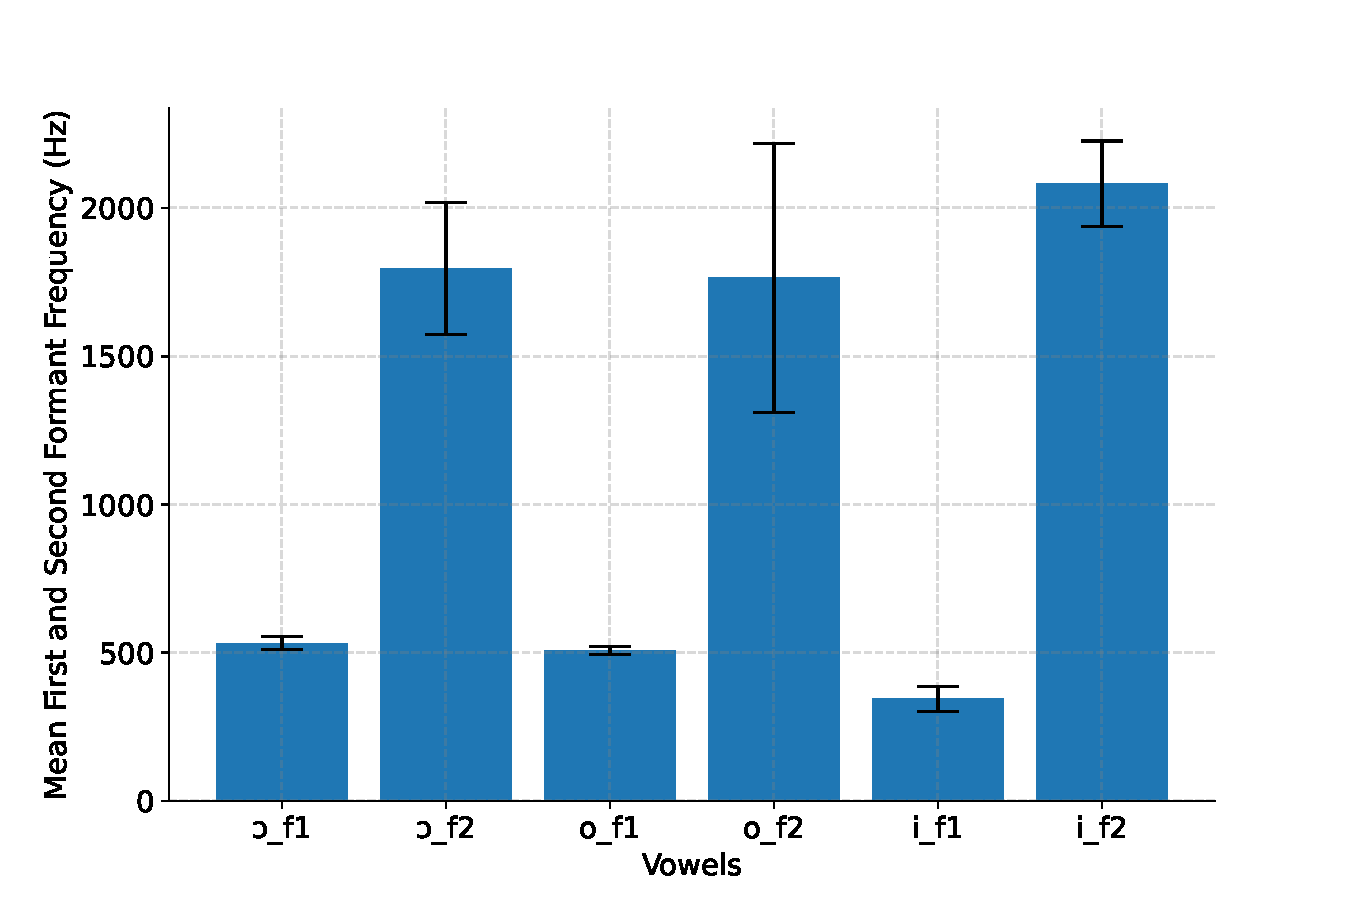
\includegraphics[width=9cm,height=5cm]{figures/IS2024_podobi_train_errorbar.pdf}};

\node[inner sep=0pt,anchor=center] (main_fig) at (10,20) % {x,y} from left corner in an imagined grid
{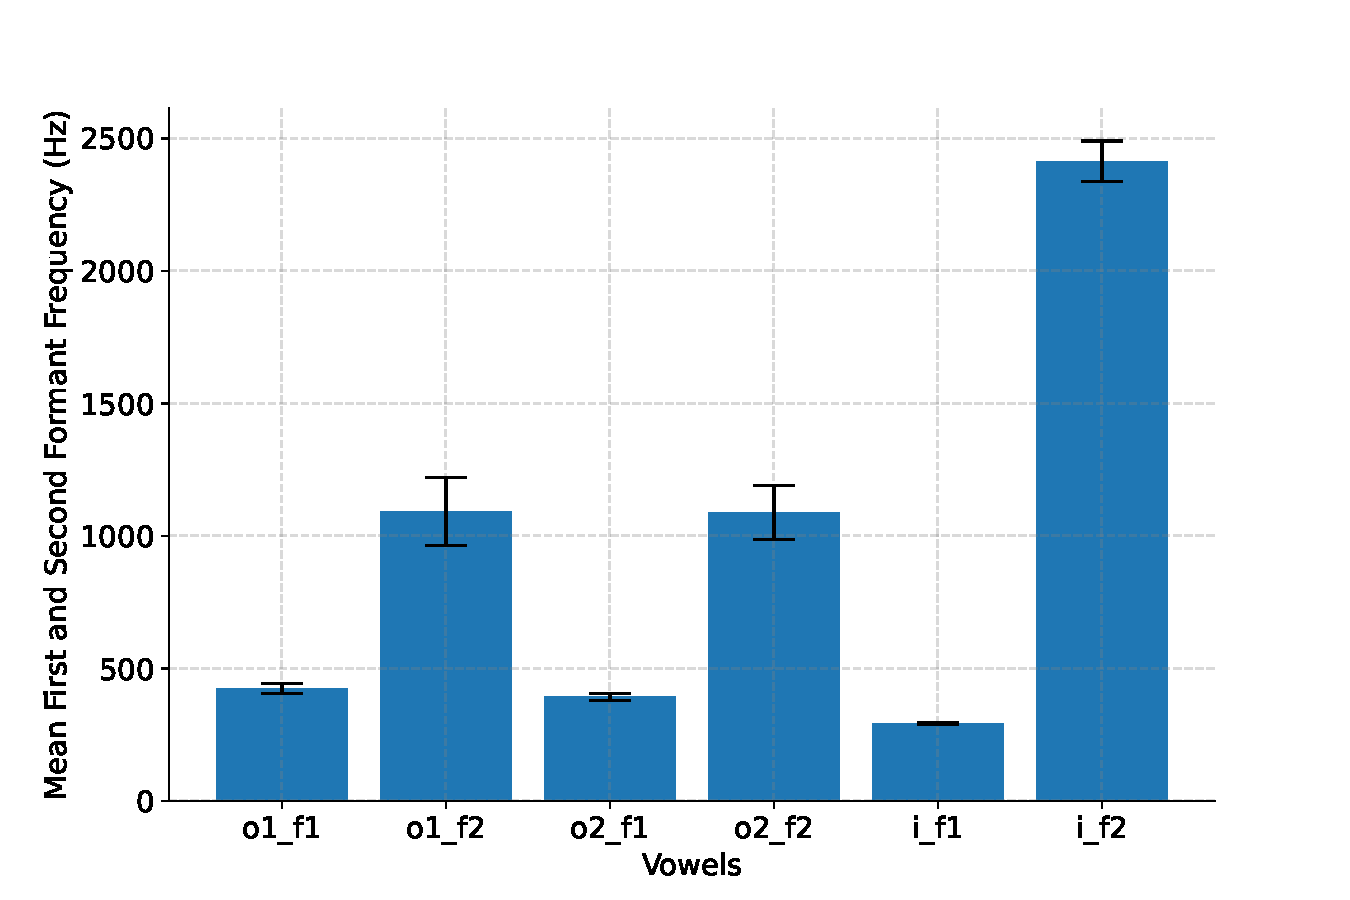
\includegraphics[width=9cm,height=5cm]{figures/IS2024_podobi_machine_errorbar.pdf}};


% ----- put axis labels
\node[font=\fontsize{8}{6}\selectfont,rotate=0,anchor=center] at (2,17.5) (l1) {(a)};
\node[font=\fontsize{8}{6}\selectfont,rotate=0,anchor=center] at (10,17.5) (l1) {(b)};

\end{tikzpicture}

    \caption{(a) First two formant frequencies of [podobi](input). (b) First two formant frequencies of [p\textopeno dobi](illicit output).}
\end{figure*}
\section{Results}
The Generator produces 100 audio files at each epoch. In the previous research in English allophonic distribution \cite{begus_identity-based_2021} and English and French nasality \cite{chen_exploring_2023}, the Generator learned to produce human speech-like sounds after 649 epochs of training, but in our case, the human-like speech was generated after 720 epochs. Intelligible sounds were generated after 800 epochs. The generated audio was manually annotated in PRAAT\cite{boersma_praat_2009} for analysis.  

After 960 epochs, the model generates lexical items identical to the training dataset ([prohori],[\textepsilon k\textepsilon b\textscripta r\textepsilon],[p\textopeno l\textopeno x]), innovative outputs([dekhisi],[korobe],[korisuw\textscripta],[debeku] etc.) as well as some illicit forms ([n\textopeno korilu], [p\textopeno dobi] etc.). We analyze the innovative outputs and observe that the model is stringing together vowels and consonants from the training data; for example, [dekhisi] is assumed to be influenced by the word [dekhisu] in the input, while [korobe] may stem from [korobi]. Since our focus of the study is vowel harmony, the vowel sequences are studied carefully in the results. The novel items [debeku], [dekhisi], and [korisuw\textscripta] follow the harmony pattern where [+high,+ATR] vowels [i,u] trigger harmony of the underlying [-ATR] vowels turning them into [+ATR]. In our above examples, we observed that [e]/[o] occurs when followed by [i]/[u] locally [korisuw\textscripta/dekhisi] as well as over a longer domain [debeku]. This suggests the model's capability to learn the phonotactics of Assamese along with iterative long-distance harmony. We further probed that vowels in the illicit items follow a specific pattern where the trigger vowels impact the immediately preceding vowel, suggesting non-iterative harmony([p\textopeno dobi] instead of [podobi]). This observation indicates the myopic nature of iterative unbounded harmony\cite{wilson_unbounded_2006}. Moreover, [korisuw\textscripta] is close to a real-world compound word [kori suw\textscripta 'do see'] and a word the model has not encountered in the input, implying the emergence of lexical learning from the training. We then examine the generated outputs statistically to examine the directionality of the vowel sequences. 

\section{Statistical analysis}
The training dataset and the generated outputs are manually annotated in PRAAT \cite{boersma_praat_2009} for quantification. We carefully examine the formant values of vowels in the training data and observe that the frequencies of the first formant (F1) of the trigger vowels are higher than the target vowels, resulting in vowel height harmony [+ATR]. We hypothesize that if V2 in the V1CV2 setting explains V1 better than V1 explains V2, the dataset follows regressive vowel harmony. If not, the directionality is assumed to be left-to-right. We conducted a linear mixed effects regression analysis \cite{bates_fitting_2015} of the training dataset in R\cite{r_core_team_r_2021} to examine the relationship between the dependent variable f1V1 and predictor variables V1 and V2 \footnote{V1full.model=lmer(f1V1$\sim$V1+V2+(1$\vert$word), data=formants, REML=FALSE)}. V1 and V2 are the fixed effects, while 'word' is the random effect in the model. The likelihood ratio test compares the full model to a null model *. The AIC score revealed a statistically significant difference between the two models (AIC(full)=1588.8, AIC(null)=1595.9). The chi-square test indicates a significant difference in model fit between the null and full models ($\chi\textsuperscript{2}$=33.062, df=13, p$<$0.001), reflecting a significant effect of V2 on the F1 value of V1. The dataset is then categorized into two subsets: harmonic and non-harmonic. Both the subsets are analyzed in the lmer model. The fixed-effects results from the full model for harmony\footnote{V1vhfull=lmer(f1V1$\sim$V1+V2+(1$\vert$word),data=har, REML=FALSE)} showed a distinction between V1, V2, and the intercept representing F1 of V1. The estimate of the intercept is about 552.129 with a p-value$<$2e-16. A comparison of the full and null model using the likelihood ratio test showed that V2 affects V1 ($\chi\textsuperscript{2}$= 27.829, df = 7, p = 0.0002361), which reveals that the contrast is statistically significant (AIC(full)=467.04, AIC(null)=480.87).  Assuming the results from statistical models for training data as a baseline, the generated items are annotated and then fit to linear regression models in R to examine the relationship between the dependent variable f1V1 and predictor variables V1 and f1V2. The model was statistically significant (F(6, 15) = 9.504, p = 0.0002087), indicating that at least one predictor variable had a non-zero effect. The Adjusted R-squared value of 0.7084 suggests that the model explained approximately 70.84\% of the variability in f1V1. The coefficients for individual predictor variables were significant at various levels. Our regression model suggests that V1 and, to some extent, f1V2 are associated with variations in f1V1.
Further analysis shows that the coefficients of V2[T.i] are significantly higher than other V2 variables (Estimate=-279.11, t-value=-3.376,p= 0.00817). This supports the idea that [i], a [+high,+ATR] vowel in Assamese, acts as a triggering vowel in the machine-generated outputs. The overall analysis suggests that the model learns the right-to-left harmony pattern, which is evident in the influence of V2 on V1 for both first and second formant frequencies.



%  \begin{figure}
%      \centering
%      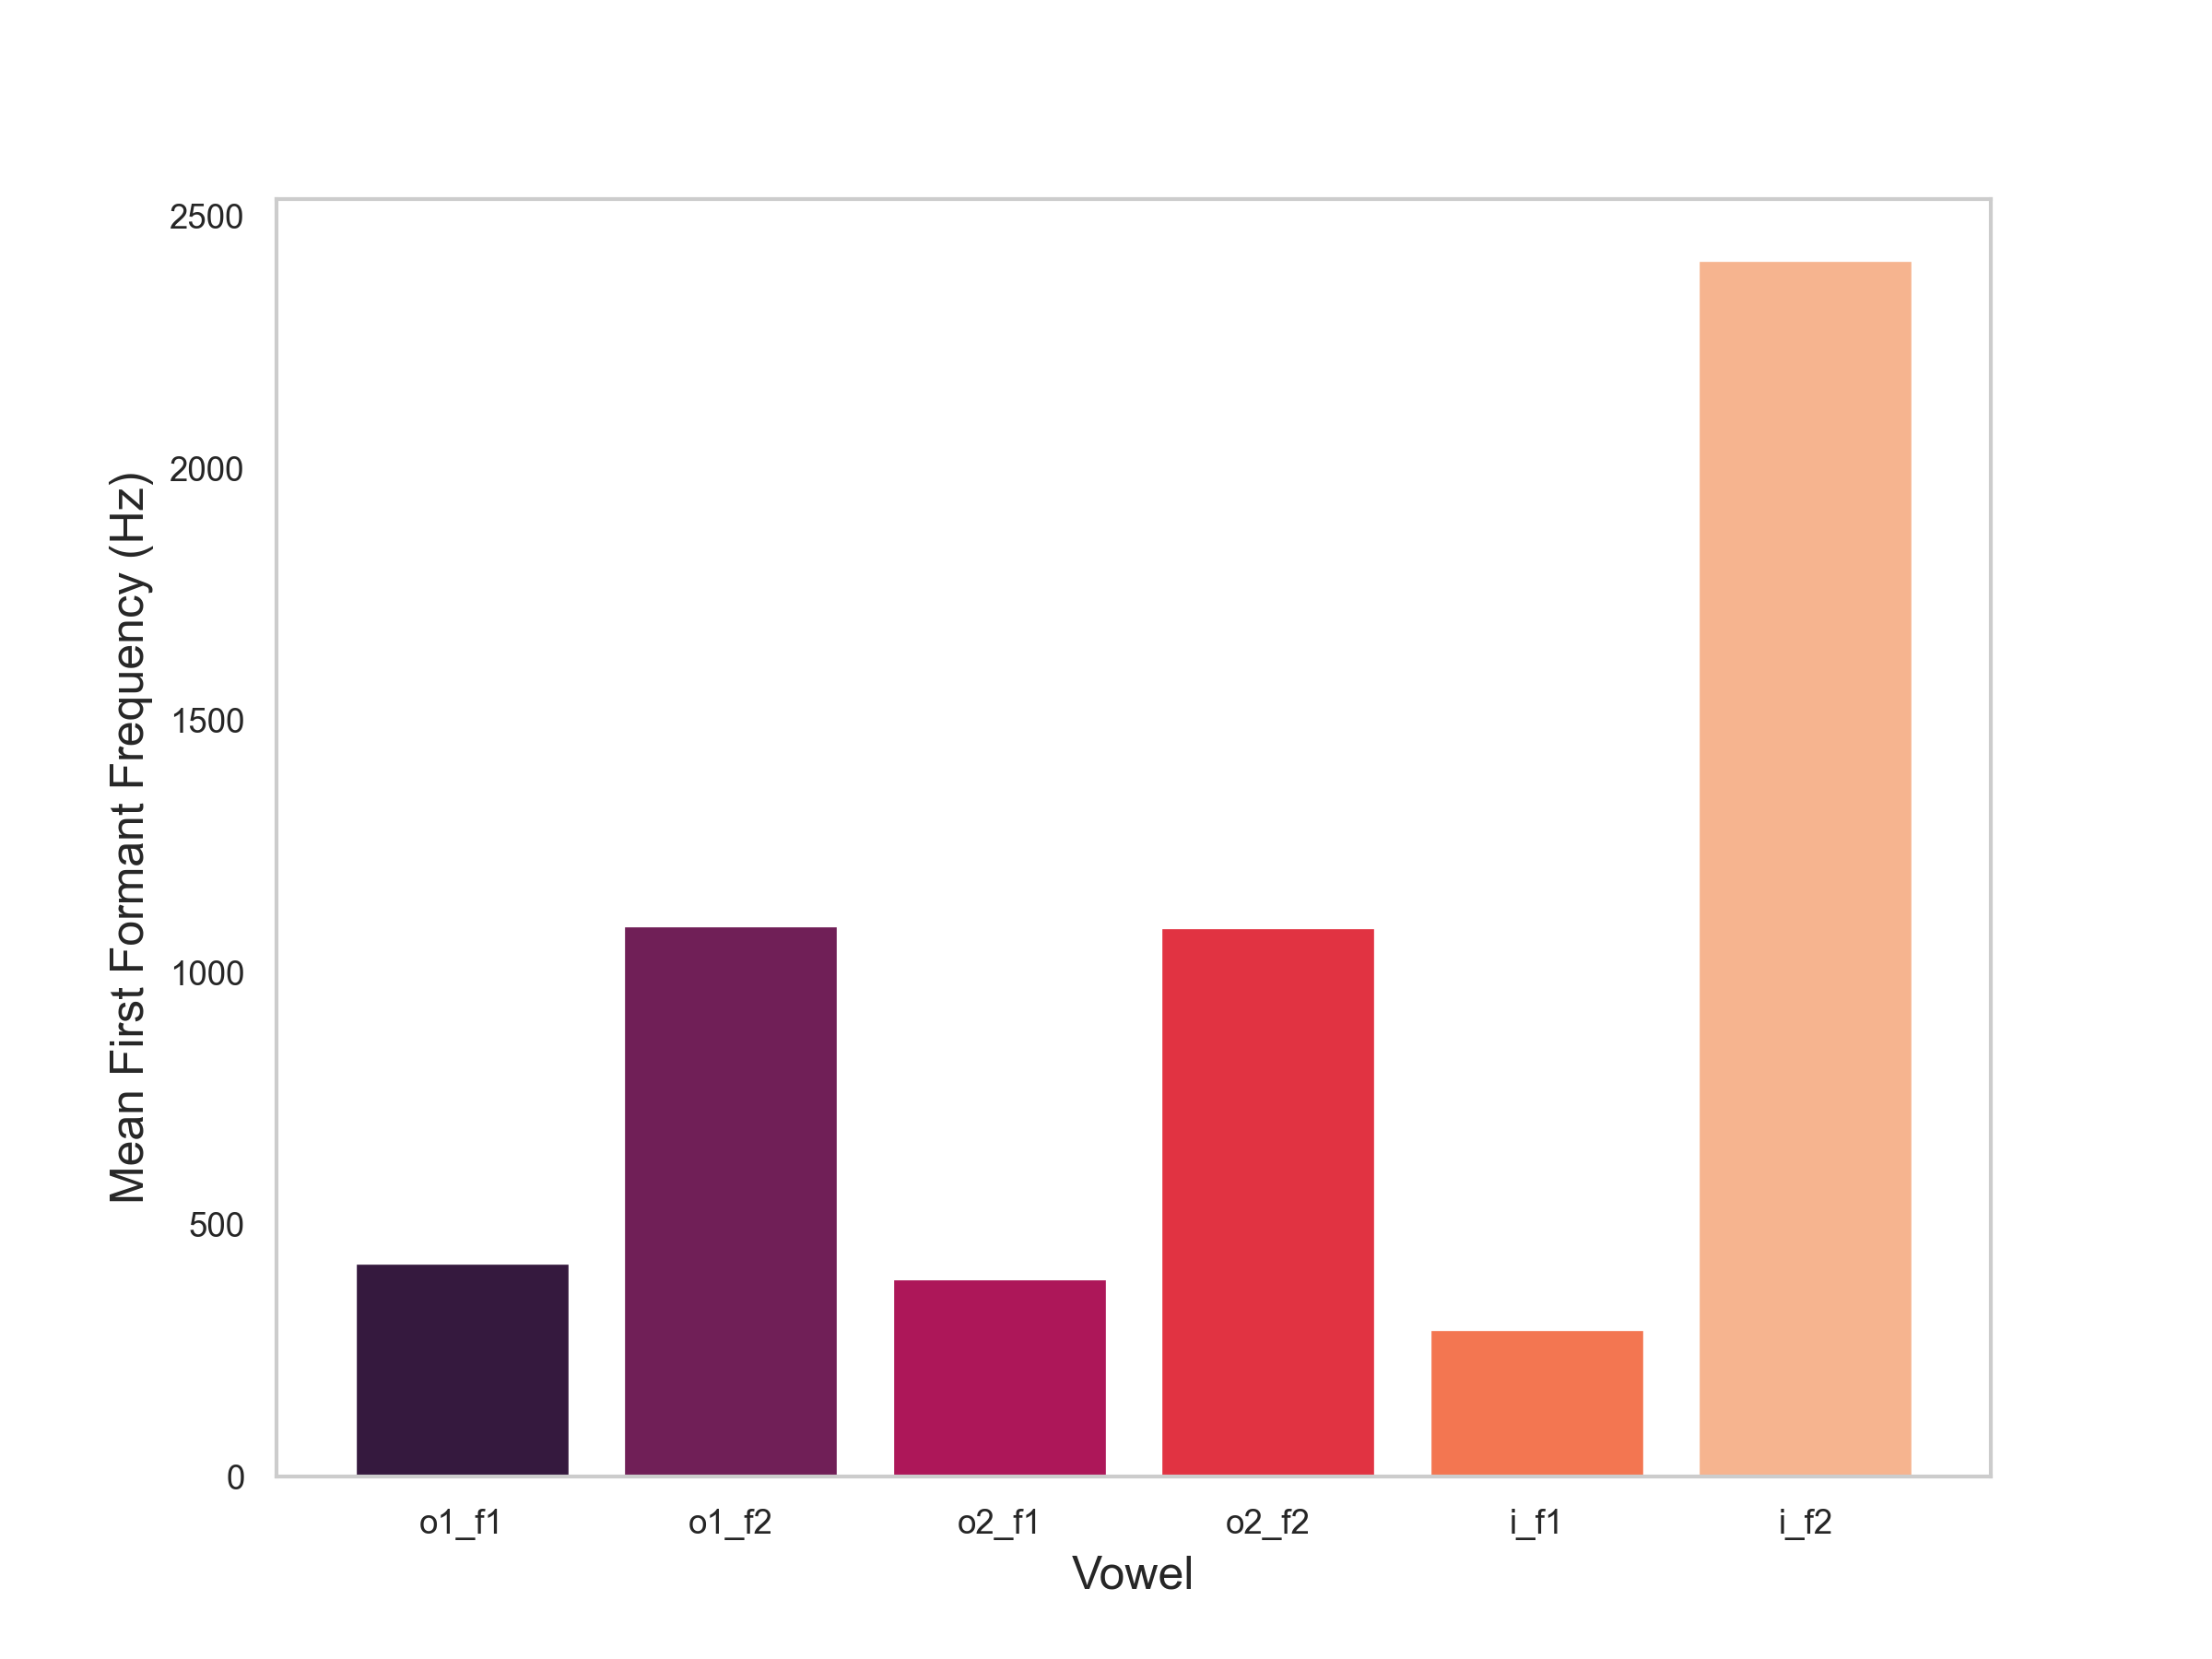
\includegraphics[width=0.5\linewidth]{podobi_train.png}
%      \caption{First two formant frequencies of [podobi](input)}
%      \label{fig:enter-label}
%  \end{figure}
 
% \begin{figure}
%     \centering
%     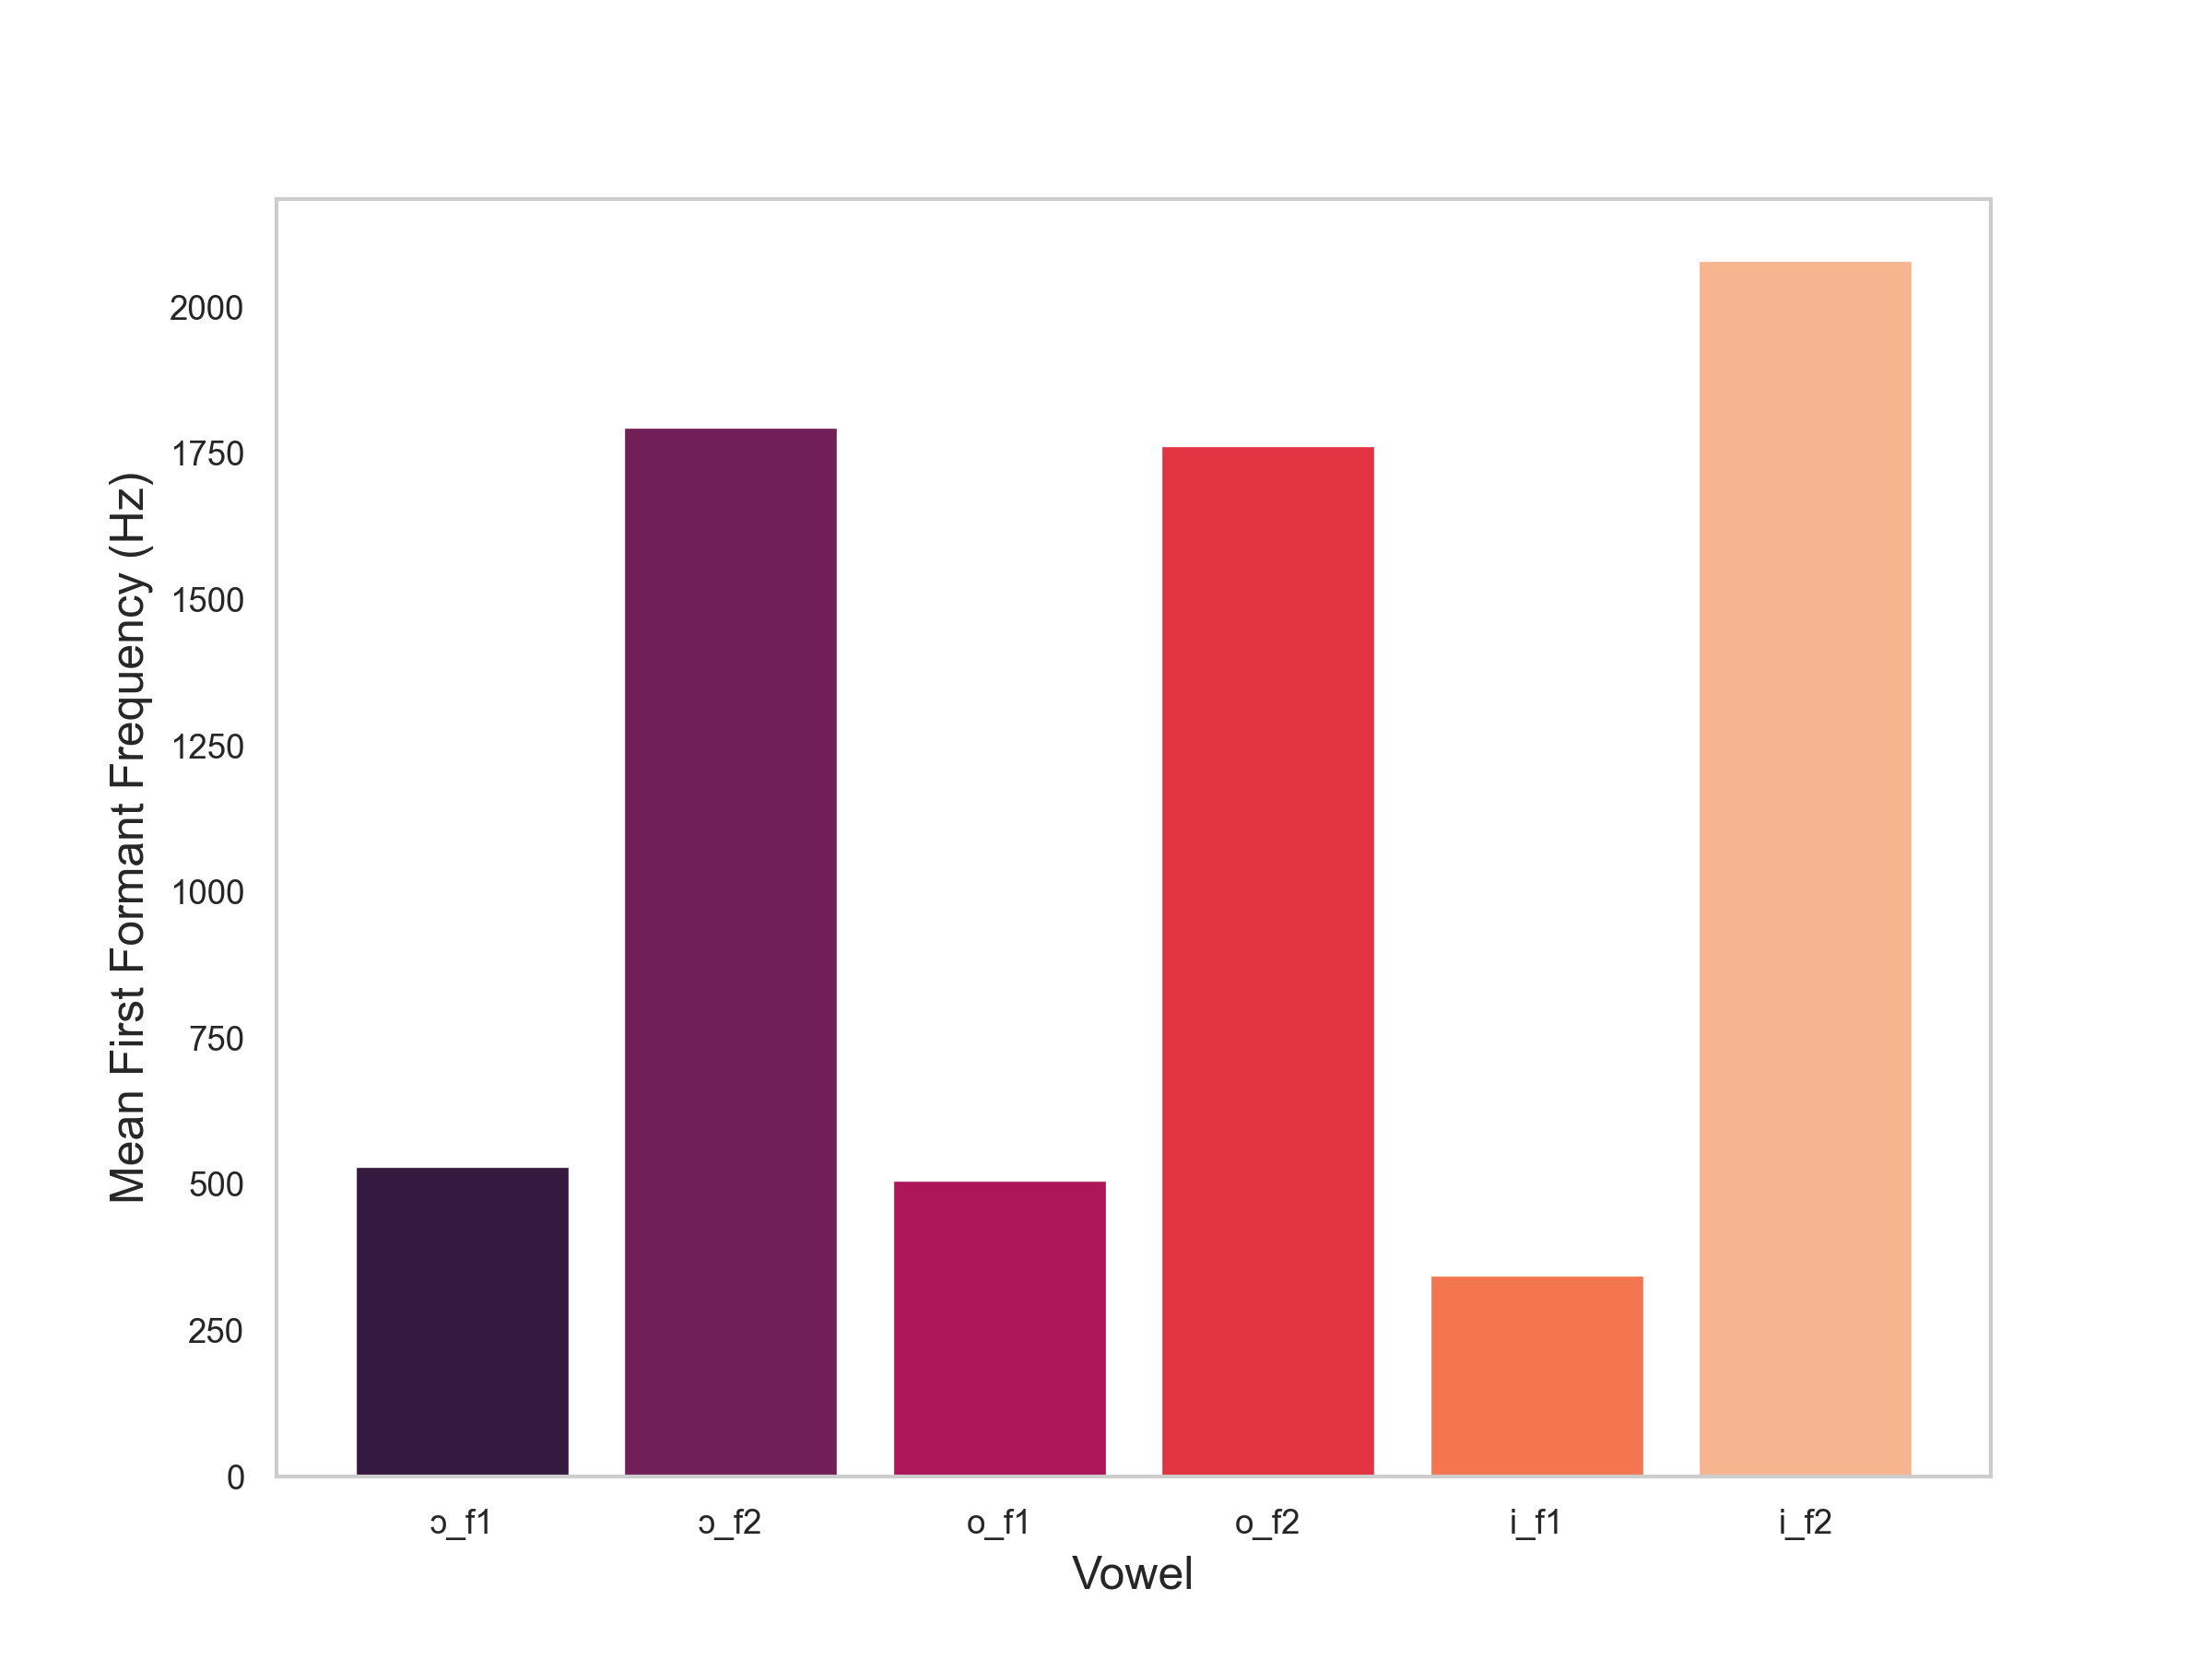
\includegraphics[width=0.5\linewidth]{podobi_machine.png}
%     \caption{First two formant frequencies of [p\textopeno dobi](illicit output)}
%     \label{fig:enter-label}
% \end{figure}


\begin{figure}
    \centering
    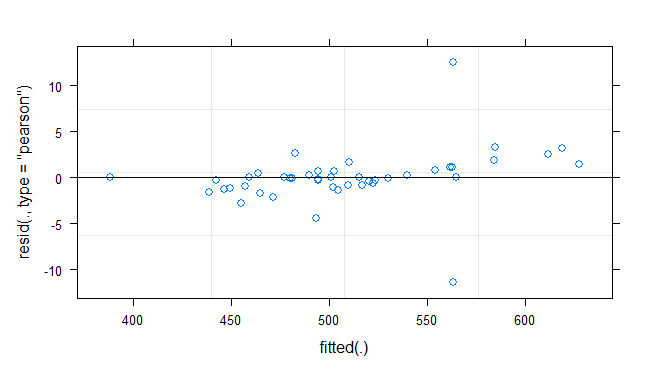
\includegraphics[width=0.75\linewidth]{lm_ATRtrain.png}
    \caption{Linear mixed effect model of right-to-left vowel harmony in Assamese}
    \label{fig:enter-label}
\end{figure}

\begin{table}[!ht]
 \caption{LMER model for the training   dataset}
    \label{tab:my_label}
    \centering
        %\adjustbox{max width=0.5\textwidth}
        \resizebox{0.5\textwidth}{!}{
    \begin{tabular}{cccccc}
    \toprule
      \textbf{Dataset type} & \textbf{Directionality} &\textbf{Fixed effects} & \textbf{DF}  &\textbf{$\chi\textsuperscript{2}$} & \textbf{p} \\
         \midrule
       Training dataset (whole) & right-to-left &bf1V1$\sim$V1+\textbf{V2} & 13  & 33.062 & $<$0.001 \\
        & left-to-right & f1V2$\sim$V2+\textbf{V1} & 10 &6.5156 & 0.7702\\
        \hline
         Training dataset ([+ATR]) & right-to-left & f1V1$\sim$V1+\textbf{V2}
& 7  & 27.829 & $<$ 0.001 \\
 & left-to-right & f1V2$\sim$V2+\textbf{V1} & 2 & 1.6522 & 0.4377\\
    \bottomrule
    \end{tabular}}
   
\end{table}

\begin{table}[!ht]
 \caption{Linear regression model for machine-generated items}
    \label{tab:my_label}
    \centering
    \adjustbox{max width=0.5\textwidth}{
    \begin{tabular}{cccc}
    \hline
        \textbf{Dataset type} & \textbf{ Estimate} & \textbf{t-value} & \textbf{p-value} \\ \hline
        Generated items (whole) & 605.25  & 7.793 & 0.0002087\\
         Generated items (V2[i]) coefficient &-279.11 & 3.376 &0.00817 \\ \hline
    \end{tabular}}
   
\end{table}
\section{Discussion and future work}

The current research explores long-distance computing of vowel patterns, emphasizing the learning of a series of vowel changes to the underlying forms required by learners to grasp vowel harmony. Much of the previous literature primarily addresses phonological learning, assuming the learner's access to grammatical forms only. Marking a crucial development for learning theories, deep learning models can generate acoustic forms exhibiting unsupervised learning of both the acoustic and articulatory properties and underlying properties like segmental features and vowel harmony. Intriguing insights into the generation of human-like speech have emerged from the extensive analysis of the Generator's performance across various epochs and manipulated latent space variables. After 960 epochs, the model demonstrated a duality: replicating known lexical items from the training set while generating novel outputs. These innovations sometimes turned out as combinations of existing words or elicited sounds, possibly due to inherent noise within the training process. It produced identical harmonic outputs as in [dekhisi] and [prohori]. Simultaneously, it also presented ungrammatical sequences ([n\textopeno korilu], [p\textopeno dobi]), akin to traditional speech errors during language acquisition. Based on our observations, we argue that given a limited quantity of data, fiwGAN is an effective phonotactic learner, as demonstrated by its novel outputs. It learns complex systems like iterative long-distance harmony. The error items show non-iterative local harmony, implying that harmony may indeed be myopic. The dominance of V2[i] as a trigger vowel indicates that the model can also learn the trigger feature. The statistical analysis further suggests that the grammatical outputs follow regressive directionality. Moreover, lexical learning emerges after the training. We did not observe any results with the opaque vowel [\textscripta], which leads us to question whether the model learns to identify vowel opacity.





\bibliographystyle{IEEEtran}
\bibliography{mybib}

\end{document}
